\documentclass[a4paper,oneside,12pt]{article}
\usepackage[slovene]{babel}
\usepackage[utf8]{inputenc}
\usepackage[T1]{fontenc}
\usepackage{url}
\usepackage{graphicx}
\usepackage[usenames]{color}
\usepackage[reqno]{amsmath}
\usepackage{amssymb,amsthm}
\usepackage{enumerate}
\usepackage{array}
\usepackage{graphicx}
\graphicspath{ {./images/} }

\usepackage[colorlinks=true,
  linkcolor=black, anchorcolor=black, citecolor=black, filecolor=black,
  menucolor=black, runcolor=black, urlcolor=black, pdfencoding=unicode,
  bookmarks=true, bookmarksopenlevel=2
]{hyperref}
\usepackage[
  paper=a4paper,
  top=2.5cm,
  bottom=2.5cm,
  textwidth=15cm,
]{geometry}

\usepackage{icomma}
\usepackage{units}
\usepackage{minted}

\newtheorem{izrek}{Izrek}
\newtheorem{posledica}{Posledica}
\theoremstyle{definition}
\newtheorem{definicija}{Definicija}
\newtheorem{opomba}{Opomba}
\newtheorem{zgled}{Zgled}

\def\R{\mathbb{R}}
\def\N{\mathbb{N}}
\def\Z{\mathbb{Z}}
\def\C{\mathbb{C}}
\def\Q{\mathbb{Q}}

\newcommand{\mytitle}{Dokumentacija za tekmovanja}
\title{\mytitle}
\author{Rok Kos}
\date{\today}
\hypersetup{pdftitle={\mytitle}}
\hypersetup{pdfauthor={Rok Kos}}
\hypersetup{pdfsubject={}}
%C++ source
\newmintedfile[cppsource]{c++}{linenos=true, mathescape, xleftmargin=0.7cm,
               fontsize=\scriptsize,baselinestretch=0.9}
%Python source
\newmintedfile[pysource]{python}{linenos=true, mathescape, xleftmargin=0.7cm,
               fontsize=\scriptsize,baselinestretch=0.9}

\newmintedfile[javasource]{java}{linenos=true, mathescape, xleftmargin=0.7cm,
			                  fontsize=\scriptsize,baselinestretch=0.9}


%----------------------------------------------------------------------------------------
%	Ostevilcevanje
\usepackage{fancyhdr}
\usepackage{lastpage}

\pagestyle{fancy}
\fancyhf{}

\rfoot{Page \thepage \hspace{1pt} of \pageref{LastPage}}

\begin{document}

%naslovnica
\thispagestyle{empty}

\vspace*{\fill}
\begin{center}
  \scalebox{3}{Dokumentacija za Izpit}\\[6ex]
  \scalebox{2}{Rok Kos}\\[4ex]
  \vfill
  verzija: \today
\end{center}

\newpage

\tableofcontents
\listoffigures

\newpage

\section{Input/Output}
	\subsection{Input}
		\javasource{IO/Input.java}
	\subsection{Output}
		\javasource{IO/Output.java}
\section{Delo s števili}
	\subsection{Parsing}
		\javasource{Stevila/Parsing.java}
	\subsection{Math knjiznica}
		\javasource{Stevila/Math.java}
	\subsection{Int/Long class}
		\javasource{Stevila/IntLong.java}
\section{Delo z besedili}
	\subsection{String class}
		\javasource{Besedila/String.java}

\section{Delo z grafiko}
	\subsection{Pravokotniki}
		Glej sliko \ref{fig:prav}\\
		\javasource{Grafika/Pravokotniki.java}
		\begin{figure}[h]
	        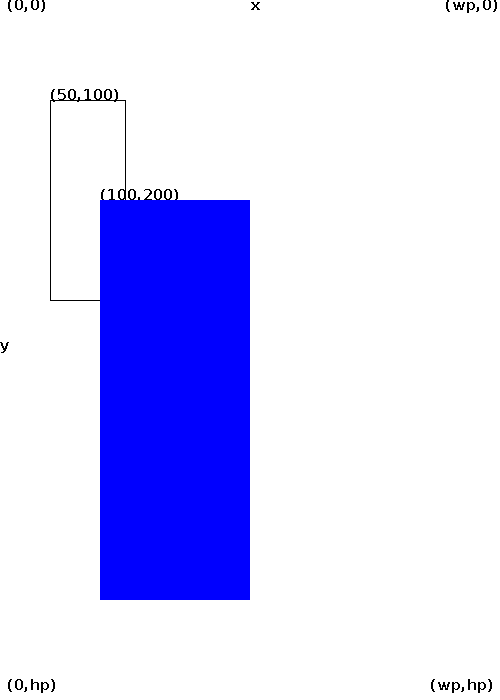
\includegraphics[width=200pt, keepaspectratio=true]{Pravokotniki.png}
	        \caption{Pravokotniki}
	        \label{fig:prav}
	    \end{figure}

	\subsection{Crte}
		Glej sliko \ref{fig:crte}\\
		\javasource{Grafika/Crte.java}
		\begin{figure}[h]
	        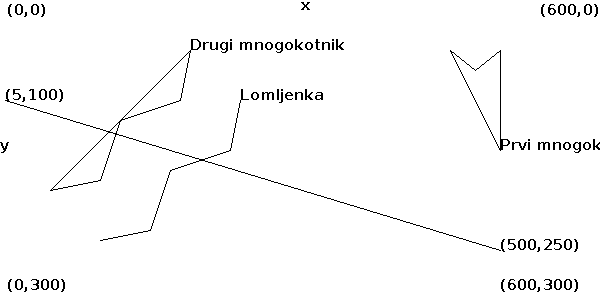
\includegraphics[width=200pt, keepaspectratio=true]{Crte.png}
	        \caption{Crte}
	        \label{fig:crte}
	    \end{figure}

		\subsection{Ovalne oblke}
			Glej sliko \ref{fig:oval}\\
			\javasource{Grafika/Krogi.java}
			\begin{figure}[h]
				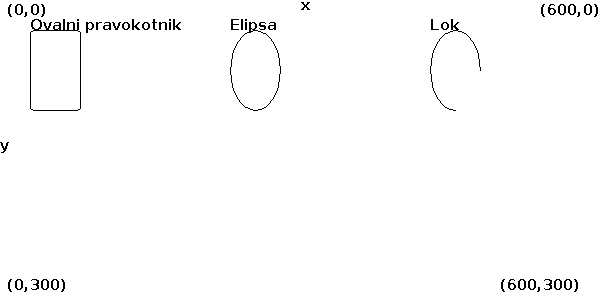
\includegraphics[width=200pt, keepaspectratio=true]{Krogi.png}
				\caption{Ovalne oblike}
				\label{fig:oval}
			\end{figure}
		\subsection{Ostalo}
			\javasource{Grafika/Ostalo.java}

\section{Razredi}
	\subsection{Primer}
		\javasource{Razredi/Primer.java}

\section{Podatkovne strukture}
	\subsection{Array}
		\javasource{PS/Array.java}
	\subsection{Queue}
		\javasource{PS/Queue.java}
	\subsection{Stack}
		\javasource{PS/Stack.java}
	\subsection{Set}
		\javasource{PS/Set.java}

\section{Algoritmi}
	\subsection{Fload Fill}
		Naloga DN09\\
		\javasource{Algo/FloadFill.java}
	\subsection{BFS}
		Naloga DN07\\
		\javasource{Algo/BFS.java}
	\subsection{Fast Power}
		Naloga DN04\\
		\javasource{Algo/FastPower.java}
\section{TJ.exe}
	\subsection{Uporaba}
		tj.exe <Program.java> <testi> <rezultati> -> normalno\\
		tj.exe <razredi> <testi> <rezultati> -> razredi\\
		tj.exe . . . -> slike\\
		tj.exe -t 5s -> cas\\
		tj.exe -p 5-10 -> primeri\\
		Rocno:\\
		javac program.java\\
		java program < input.txt > output.txt\\
		(java Program rezultat.png 700x500 za slike)\\
		fc output.txt pravilno.txt (Linux/Mac diff)\\




\end{document}
